\section{Is Platt scaling calibrated?}
\label{sec:challenges-measuring}

In this section, we show why methods like Platt scaling and temperature scaling are (i) less calibrated than reported and (ii) it is difficult to tell how miscalibrated they are. The issue is that it is very difficult to measure the calibration error of models that output a continuous range of values. We show, both theoretically and with experiments on CIFAR-10 and ImageNet, why the calibration error of such models is \emph{underestimated}. We defer proofs to the Appendix.

% We begin by reviewing the definition of uncertainty calibration in the binary classification setting. Let $\mathcal{X} \subseteq \mathbb{R}^d$ and $\mathcal{Y} = \{0, 1\}$. Let $X \in \mathcal{X}$ and $Y \in \mathcal{Y}$ be random variables denoting the input and label, given by an unknown joint distribution $P(X, Y)$. Suppose we have a model $f : \mathcal{X} \to [0, 1]$ where the output of the model represents the model's confidence that the label is 1.

% \begin{definition}
% A model $f : \mathcal{X} \to [0, 1]$ is perfectly calibrated if $s = E[Y | f(X) = s]$ for all $s \in [0, 1]$.
% \end{definition}

% \begin{definition}
% For $p \geq 1$, the $\ell_p$ calibration error of a model $f : \mathcal{X} \to [0, 1]$ is given by:
% \[ \ell_p\mbox{-CE}(f) = \Big(E\big[ (f(X) - E[Y | f(X)])^p \big] \Big)^{1/p} \]
% \end{definition}

% The $\ell_2^2$, $\ell_1$ and $\ell_{\infty}$ calibration errors are popular choices. For all $p$, the $\ell_p$ calibration error can be tricky to estimate from samples, because $E[Y | f(X)]$ is difficult to estimate. In particular, for a model $f$ that outputs a continuous range of values between $[0, 1]$, we usually see any given $f(X)$ value exactly once.
% This makes estimating $E[Y | f(X)$ impossible without additional assumptions on the smoothness of $E[Y | f(X)]$.

For all $p$, the $\ell_p$ calibration error can be tricky to estimate from samples, because $E[Y \; | \; f(X)]$ is difficult to estimate.
In particular, for a model $f$ that outputs a continuous range of values between $[0, 1]$, we usually see any given $f(X)$ value exactly once.
To approximate the $\ell_p$ calibration error, prior work bins the output space $f(X)$ into $B$ intervals.
The calibration error in each bin is estimated as the difference between the average value of $f(X)$ and $Y$ in that bin, as defined below.

\begin{definition}
A binning scheme $\mathcal{B}$ is a set of $B$ disjoint intervals $I_1, \cdots, I_B$ that cover $[0, 1]$.
\end{definition}

\begin{definition}
Given a model $f : \mathcal{X} \to [0, 1]$ and a binning scheme $\mathcal{B}$, for any interval $I_j \in \mathcal{B}$ let:
\[ \bar{f}(I_j) = E[f(X) | f(X) \in I_j] \]
\[ \bar{Y}(I_j) = E[Y | f(X) \in I_j] \]
Then the binned $\ell_p$ calibration error is given by:
\[ \ell_p\mbox{-CE}(f, B) = \Big( \sum_{j=1}^B P(f(X) \in I_j) \left|\bar{f}(I_j) - \bar{Y}(I_j) \right|^p  \Big)^{1/p} \]
\end{definition}
\tm{I am not sure we need this definition. does it suffice to talk about the calibration error of the binned function, and say that's what people are doing? Or at least it seems that the notion above should be defined through the calibration error of the binned function}

A simple example shows that the binned $\ell_p$ calibration error can severely underestimate the true $\ell_p$ calibration error, even for $p=1$, the average calibration error.

\begin{restatable}{example}{continuousNotCalibrated}
\label{ex:continuous-not-calibrated}
For any binning scheme $\mathcal{B}$, $p \in \mathbb{Z}^+$, and continuous surjective function $f : \mathcal{X} \to [0, 1]$, there exists a distribution $P$ over $X, Y$ s.t. $\ell_p\mbox{-CE}(f, \mathcal{B}) = 0$ but $\ell_p\mbox{-CE}(f) = 0.5$.
Note that for all $f$, $0 \leq \ell_p\mbox{-CE}(f) \leq 1$.
\end{restatable}

% \begin{proof}
% The intuition is that $E[Y | f(X)]$ can be a function that oscillates a lot (like a sine wave with very high frequency), but for each interval $I_j$ we still have $\hat{f}(I_j) = \hat{Y}(I_j)$. Formal proof in Appendix.
% \end{proof}

The construction, in the Appendix, is perhaps contrived, but we will show experimental evidence of this phenomena as well. Next, we show that the binned $\ell_p$ calibration error is a lower bound of the true $\ell_p$ calibration error, and that \emph{finer} binning schemes give us a better lower bound.

\begin{definition}
Let $\mathcal{B}$ given by intervals $I_1, ..., I_m$ and $\mathcal{B}'$ given by intervals $I_1', ..., I_n'$ be binning schemes. We say $\mathcal{B}' \preceq \mathcal{B}$ if for all $1 \leq j \leq n$, there exists $1 \leq k \leq m$ s.t. $I_j' \subseteq I_k$. 
\end{definition}

% \begin{example}
% A finer binning scheme partitions $[0, 1]$ into a finer set of intervals. If $\mathcal{B}_1 = \{ (0, 0.5), (0.5, 1.0)\}$ and $\mathcal{B}_2 = \{(0, 0.2), (0.2, 0.5), (0.5, 0.75), (0.75, 1.0)\}$, then we $\mathcal{B}_2$ is a finer binning scheme than $\mathcal{B}_1$. On the other hand, $\mathcal{B}_3 = \{(0, 0.2), (0.2, 0.6), (0.6, 1.0)\}$ is not a finer binning scheme than $\mathcal{B}_1$. 
% \end{example}

\begin{restatable}[Binning underestimates error]{proposition}{binningLowerBound}
Given $\bins{}' \preceq \bins{}$ and model $f : \mathcal{X} \to [0, 1]$. We have:
\[  \ell_p\mbox{-CE}(f, \bins{}) \leq \ell_p\mbox{-CE}(f, \bins{}') \leq \ell_p\mbox{-CE}(f) \]
\end{restatable}

\subsection{Experiments}

To see if this phenomena occurs in practice, we ran experiments on CIFAR-10 and Imagenet, which show that increasing the number of bins uncovers a higher model calibration error.
The model's objective was to output the top predicted class and a confidence score associated with the prediction.
For CIFAR-10, we used a trained VGG-net model with an accuracy of 93.1\%.
We then split the test set into 3 chunks of size $(1000, 1000, 8000)$.
We used the first chunk of data to recalibrate the model using Platt Scaling, the second to select the binning scheme $\mathcal{B}$, and the third to measure the binned calibration error.
We calculated $90\%$ confidence intervals for the binned calibration error using 1,000 Bootstrap resamples.
We performed the same experiment with varying numbers of bins --
the results are shown in Figure~\ref{fig:lower_bounds}. We repeated this experiment on ImageNet using a trained VGG-net model with top-1 accuracy of 64.3\%, splitting the validation set into 3 chunks of size $(20000, 5000, 25000)$.
In the Appendix we show that similar results hold for the $\ell_1$ calibration error as well.

\begin{figure}
     \centering
     \begin{subfigure}[b]{0.47\textwidth}
         \centering
         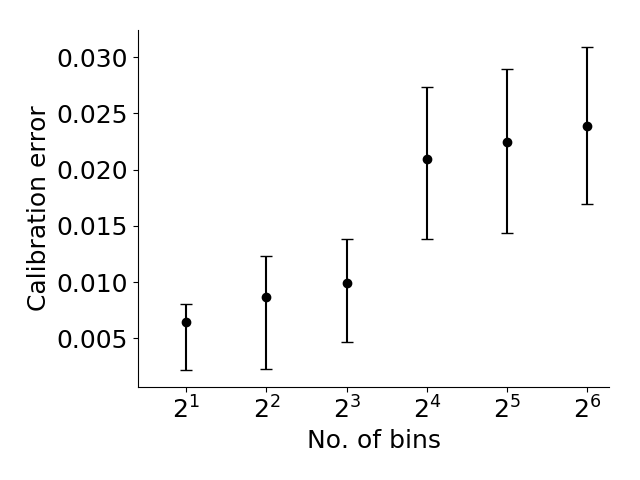
\includegraphics[width=\textwidth]{lower_bound_cifar_plot}
         \caption{CIFAR-10.}
         \label{fig:cifat_10_lower_bound}
     \end{subfigure}
     \hfill
     \begin{subfigure}[b]{0.47\textwidth}
         \centering
         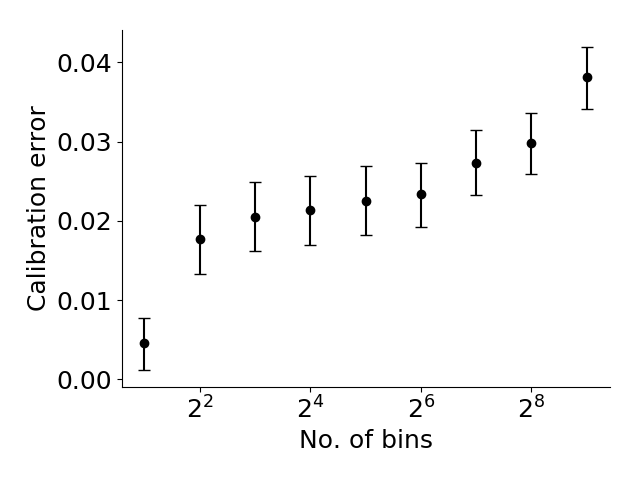
\includegraphics[width=\textwidth]{lower_bound_imagenet_plot}
         \caption{ImageNet.}
         \label{fig:imagenet_lower_bound}
     \end{subfigure}
        \caption{
        Binned $\ell_2$ calibration errors of a recalibrated VGG-net model on CIFAR-10 and ImageNet with $90\%$ confidence intervals. The binned calibration error increases as we increase the number of bins. This suggests that binning cannot be reliably used to measure the true calibration error.
        }
        \label{fig:lower_bounds}
\end{figure}


% We might also wish to compare the calibration of different candidate models.
Our experiments suggest that the binned calibration error gives us a poor sense of a model's calibration error if the model outputs a continuous range of values.
% \footnote{One possibility is to modify the calibration metric, for example to only require our model to be calibrated for all possible intervals of width $\geq \epsilon$.}

% One possibility is to modify the calibration metric, for example to only require our model to be calibrated for all possible intervals of width $\geq \epsilon$. 
% % This makes it difficult to ascertain if a model has a desired calibration error, or which of two models is better calibrated.

% We see three potential ways to resolve this:
% \begin{enumerate}
% \item Add a smoothness constraint on $E[Y | f(X)$], for example assume $E[Y | f(X)]$ is $L$-Lipschitz. Smoothness assumptions are common when training a model, but it is unsatisfying to assume a value of $L$, which we do not know, when \emph{evaluating} a model.
% \item Explore alternative metrics for calibration. For example, perhaps we only require our model to be calibrated for all possible intervals of width $\geq \epsilon$. 
% \item Discretize the outputs of the final model, so that it only outputs a finite number of values.
% \end{enumerate}

% In this paper we explore (3), but (1) and (2) are good directions for future research.

